\documentclass[tikz, border=10pt]{standalone}

\begin{document}
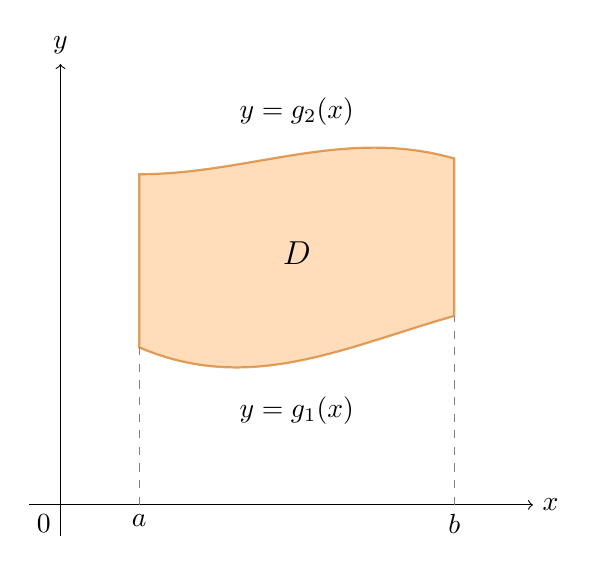
\begin{tikzpicture}[scale=2]

    % Define boundaries based on the image's appearance
    \def\a{0.5}
    \def\b{2.5}
    \def\ymax{2.3}

    % Define coordinates for bezier paths that mimic the general shape
    \coordinate (A1) at (\a, 1.0); % Start of g1
    \coordinate (A2) at (\a, 2.1); % Start of g2
    \coordinate (B1) at (\b, 1.2); % End of g1
    \coordinate (B2) at (\b, 2.2); % End of g2

    % Draw the boundary and shade the region D using a single path command
    \draw[orange!80!black, thick, fill=orange!45, opacity=0.6] 
        (A1) .. controls (1.2, 0.7) and (1.8, 1.0) .. (B1) -- 
        (B2) .. controls (1.8, 2.4) and (1.2, 2.1) .. (A2) -- cycle;

    % Draw axes
    \draw[->] (-0.2, 0) -- (\b+0.5, 0) node[right] {$x$};
    \draw[->] (0, -0.2) -- (0, \ymax+0.5) node[above] {$y$};
    \node[below left] at (0,0) {$0$};

    % Draw the dashed vertical lines down to x-axis
    \draw[dashed, gray] (\a, 0) -- (\a, 1.0);
    \draw[dashed, gray] (\b, 0) -- (\b, 1.2);

    % Label a and b on the x-axis
    \node[below] at (\a, 0) {$a$};
    \node[below] at (\b, 0) {$b$};

    % Label the functions
    \node[above] at (1.5, 2.35) {$y=g_2(x)$};
    \node[below] at (1.5, 0.75) {$y=g_1(x)$};

    % Label the region D
    \node[font=\large] at (1.5, 1.6) {$D$};

\end{tikzpicture}
\end{document}
